\chapter{Projekt bazy danych i model danych}
\label{chap:baza-danych}

\section{Założenia modelu danych}

Baza danych systemu \textit{IdentityCore} została zaprojektowana jako relacyjny model danych przechowujący informacje potrzebne do działania lokalnego systemu identyfikacji osób. Jej zadaniem jest uporządkowane zapisanie danych osób, danych biometrycznych, historii prób identyfikacji, ustawień systemowych oraz danych technicznych związanych z logowaniem operatora.

Jednym z głównych założeń modelu jest oddzielenie danych osoby od danych biometrycznych. Dane opisowe osoby są przechowywane w tabeli \texttt{Persons}, natomiast dane wykorzystywane przez identyfikację twarzy i odcisku palca znajdują się w osobnych tabelach. Dzięki temu jedna osoba może być powiązana z wieloma rekordami biometrycznymi, a podstawowy rejestr osób nie musi przechowywać wszystkich danych technicznych związanych z biometrią.

Historia prób identyfikacji została wydzielona do tabeli \texttt{IdentificationAttempts}. Dodatkowe wyniki dopasowań kandydatów są przechowywane w tabeli \texttt{MatchResults}. Takie rozdzielenie pozwala zapisać zarówno ogólny wynik próby, jak i szczegółowe informacje o kandydatach uzyskanych podczas porównania.

Ustawienia systemowe są przechowywane w tabeli \texttt{SystemSettings}. Są one niezależne od konkretnych osób, ponieważ dotyczą konfiguracji działania aplikacji. Dane operatora aplikacji znajdują się w tabeli \texttt{Users}, która służy do obsługi technicznego logowania do systemu.

Przyjęty model danych ułatwia utrzymanie informacji, testowanie aplikacji oraz dalszą rozbudowę systemu. Oddzielne tabele dla osób, danych biometrycznych, prób identyfikacji i ustawień pozwalają rozwijać poszczególne części aplikacji bez mieszania różnych typów danych w jednej strukturze.

\section{Opis głównych encji}

Główne encje modelu danych odpowiadają najważniejszym obszarom działania aplikacji: rejestrowi osób, danym biometrycznym, historii prób, ustawieniom oraz logowaniu operatora. Zestawienie tabel przedstawiono w tabeli~\ref{tab:glowne-tabele-bazy}.

\setlength{\tabcolsep}{4pt}
\renewcommand{\arraystretch}{1.15}
\begin{xltabular}{\textwidth}{|
    >{\RaggedRight\arraybackslash}p{4.6cm}|
    >{\RaggedRight\arraybackslash}X|}

    \hline
    \textbf{Tabela} & \textbf{Rola w systemie} \\
    \hline
    \endfirsthead

    \hline
    \textbf{Tabela} & \textbf{Rola w systemie} \\
    \hline
    \endhead

    \texttt{Users} & Przechowuje dane techniczne operatora aplikacji, takie jak nazwa użytkownika, hasło, imię i nazwisko, rola, aktywność konta oraz data utworzenia. Tabela służy do obsługi logowania. \\
    \hline
    \texttt{SystemSettings} & Przechowuje ustawienia systemowe w postaci klucza, wartości, opisu i daty aktualizacji. Tabela służy do przechowywania parametrów konfiguracyjnych. \\
    \hline
    \texttt{Persons} & Przechowuje podstawowe dane osób zarejestrowanych w systemie, w tym kod osoby, imię, nazwisko, dane opisowe, status oraz ścieżki do obrazów profilowych i biometrycznych. \\
    \hline
    \texttt{FaceTemplates} & Przechowuje szablony twarzy powiązane z osobami. Zawiera m.in. identyfikator osoby, ścieżkę do obrazu źródłowego, zapis embeddingu, ocenę jakości, nazwę modelu. \\
    \hline
    \texttt{FingerprintTemplates} & Przechowuje szablony odcisków palców powiązane z osobami. Zawiera m.in. identyfikator osoby, pozycję palca, ścieżkę do obrazu źródłowego, dane szablonu, ocenę jakości, nazwę algorytmu, rozdzielczość DPI. \\
    \hline
    \texttt{BiometricSamples} & Przechowuje informacje o próbkach biometrycznych przypisanych do osób. Tabela zawiera typ biometrii, ścieżkę do pliku, ocenę jakości, notatki oraz datę utworzenia. \\
    \hline
    \texttt{IdentificationAttempts} & Przechowuje historię prób identyfikacji. Zawiera datę próby, typ biometrii, ścieżkę do pliku wejściowego, najlepiej dopasowaną osobę, wynik podobieństwa, decyzję, operatora oraz status próby. \\
    \hline
    \texttt{MatchResults} & Przechowuje wyniki kandydatów powiązane z konkretną próbą identyfikacji. Tabela zapisuje kilku wyników dopasowania, ich kolejności, decyzji oraz powiązania z osobą. \\
    \hline

    \caption{Główne tabele bazy danych systemu IdentityCore}
    \label{tab:glowne-tabele-bazy}
\end{xltabular}

\setlength{\tabcolsep}{6pt}

Model danych obejmuje zarówno tabele bezpośrednio związane z identyfikacją biometryczną, jak i tabele pomocnicze. Dzięki temu baza danych przechowuje dane osób, szablony, ustawienia, historię prób oraz wyniki kandydatów.

\section{Relacje między tabelami}

Centralną rolę w modelu danych pełni tabela \texttt{Persons}. To z nią powiązane są dane biometryczne twarzy, dane biometryczne odcisków palców oraz próbki biometryczne. Relacje te pozwalają przypisać wiele rekordów biometrycznych do jednej osoby.

Tabela \texttt{FaceTemplates} posiada klucz obcy \texttt{PersonId} wskazujący na tabelę \texttt{Persons}. Relacja ta wykorzystuje regułę \texttt{ON DELETE CASCADE}, co oznacza, że usunięcie osoby powoduje usunięcie powiązanych szablonów twarzy. Analogicznie tabela \texttt{FingerprintTemplates} posiada klucz obcy \texttt{PersonId} wskazujący na tabelę \texttt{Persons} również z regułą \texttt{ON DELETE CASCADE}.

Tabela \texttt{BiometricSamples} także jest powiązana z tabelą \texttt{Persons} przez pole \texttt{PersonId}. Dzięki temu próbki biometryczne nie funkcjonują jako niezależne rekordy, lecz są przypisane do konkretnej osoby.

Tabela \texttt{IdentificationAttempts} przechowuje informacje o wykonanych próbach identyfikacji. Pole \texttt{BestMatchPersonId} wskazuje na osobę najlepiej dopasowaną podczas próby. Relacja z tabelą \texttt{Persons} wykorzystuje regułę \texttt{ON DELETE SET NULL}, dlatego usunięcie osoby nie usuwa historii próby, lecz zeruje powiązanie z osobą. Pozwala to zachować zapis historii nawet wtedy, gdy rekord osoby zostanie usunięty.

Tabela \texttt{MatchResults} jest powiązana z tabelą \texttt{IdentificationAttempts} przez pole \texttt{IdentificationAttemptId}. Zastosowano tutaj regułę \texttt{ON DELETE CASCADE}, więc usunięcie próby identyfikacji usuwa również powiązane wyniki kandydatów. Tabela \texttt{MatchResults} może być też powiązana z tabelą \texttt{Persons} przez pole \texttt{PersonId}. W tym przypadku zastosowano regułę \texttt{ON DELETE NO ACTION}.

\section{Diagram ERD}

Diagram ERD przedstawia graficzne ujęcie tabel oraz relacji występujących w modelu danych. Obejmuje on przede wszystkim powiązania tabel \texttt{Persons}, \texttt{FaceTemplates}, \texttt{FingerprintTemplates}, \texttt{BiometricSamples}, \texttt{IdentificationAttempts} oraz \texttt{MatchResults}. Tabele \texttt{SystemSettings} i \texttt{Users} pełnią funkcje pomocnicze i również zostały uwzględnione w modelu.

\begin{figure}[H]
    \centering
    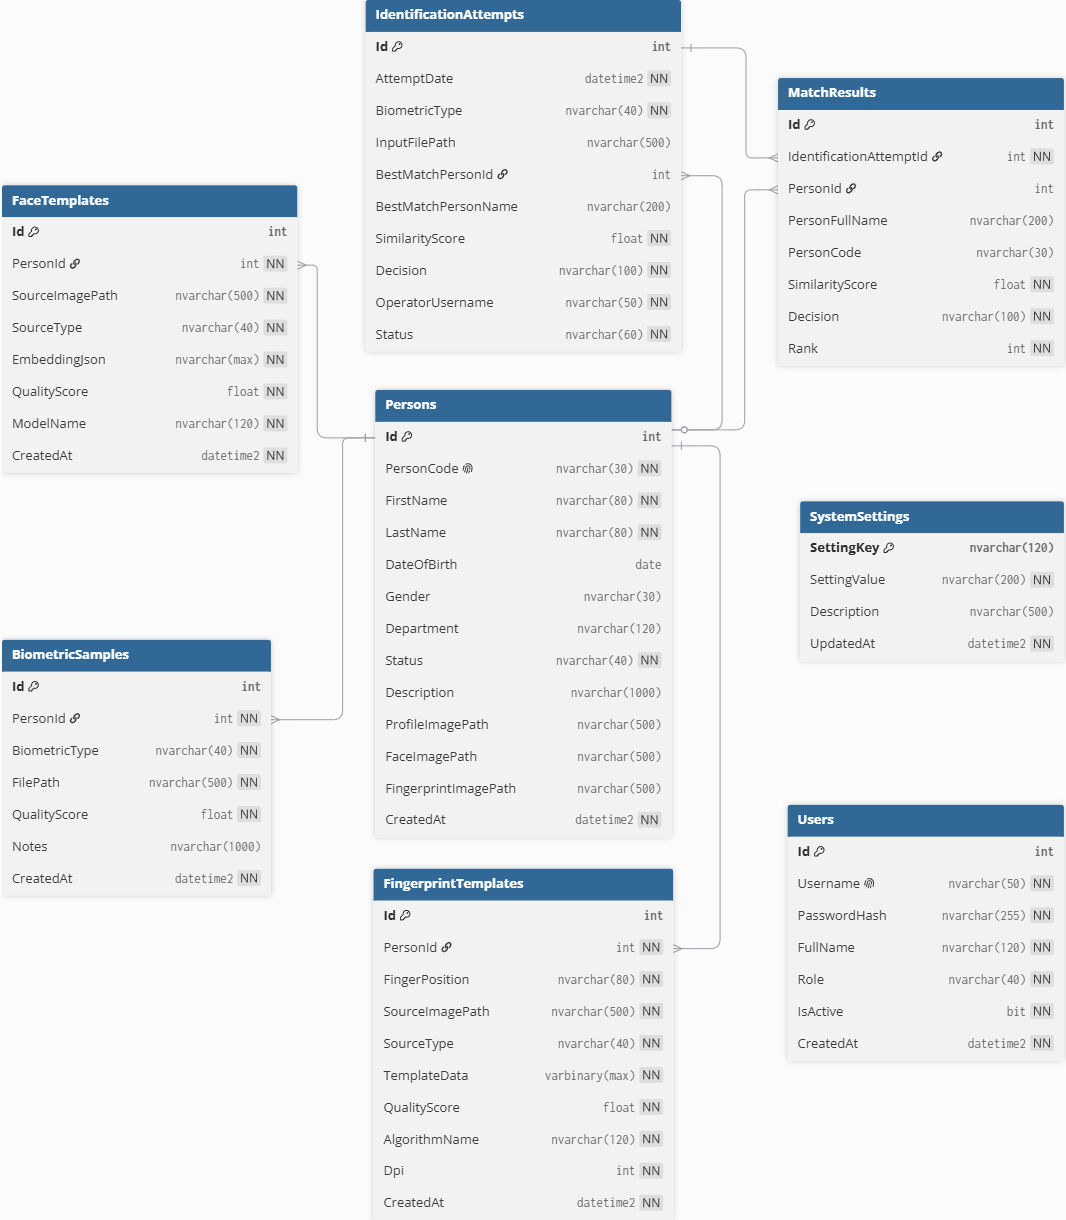
\includegraphics[width=\textwidth]{figures/erd_identitycore.png}
    \caption{Diagram ERD bazy danych systemu IdentityCore}
    \label{fig:erd-identitycore}
\end{figure}

Diagram ułatwia zrozumienie, które tabele stanowią centrum modelu danych oraz w jaki sposób rekordy biometryczne i historia prób są powiązane z osobami zarejestrowanymi w systemie.

\section{Integralność danych}

Integralność danych w bazie wynika przede wszystkim z zastosowania kluczy głównych, kluczy obcych, ograniczeń unikalności oraz wartości domyślnych. Większość głównych tabel posiada klucz główny \texttt{Id} typu całkowitego z automatycznym nadawaniem wartości. Wyjątkiem jest tabela \texttt{SystemSettings}, w której kluczem głównym jest \texttt{SettingKey}.

W tabeli \texttt{Persons} zastosowano unikalny kod osoby zapisany w kolumnie \texttt{PersonCode}. Tabela \texttt{Users} posiada unikalną nazwę użytkownika w kolumnie \texttt{Username}. Ograniczenia te zmniejszają ryzyko duplikowania rekordów o tym samym identyfikatorze logicznym.

Klucze obce wiążą dane biometryczne z osobami oraz wyniki dopasowań z próbami identyfikacji. Tabele \texttt{FaceTemplates}, \texttt{FingerprintTemplates} i \texttt{BiometricSamples} odnoszą się do tabeli \texttt{Persons}, natomiast tabela \texttt{MatchResults} odnosi się do tabeli \texttt{IdentificationAttempts}. Dzięki temu szablony i wyniki nie są przechowywane jako całkowicie oderwane dane.

Oddzielenie danych osób od danych biometrycznych ogranicza duplikację informacji. Dane opisowe osoby nie muszą być powtarzane przy każdym szablonie twarzy lub odcisku palca. W przypadku dodania kolejnych próbek lub szablonów wystarczy utworzyć nowe rekordy powiązane z istniejącą osobą.

\section{Skrypty bazy danych i migracje}

W projekcie zastosowano trzy główne skrypty SQL przechowywane w katalogu \texttt{Database}. Ich zadaniem jest przygotowanie bazy danych, aktualizacja starszej struktury oraz czyszczenie danych biometrycznych podczas testów.

Plik \texttt{create\_database.sql} służy do utworzenia bazy \texttt{IdentityCoreDb} od podstaw. Skrypt tworzy pełną aktualną strukturę tabel, usuwa wcześniej istniejące tabele aplikacji, zakłada klucze, relacje oraz indeksy, a także dodaje podstawowe dane startowe i domyślne ustawienia decyzyjne. Jest to skrypt przeznaczony do świeżej instalacji albo świadomego odtworzenia bazy od zera.

Plik \texttt{update\_existing\_database.sql} służy do aktualizacji starszej istniejącej bazy bez usuwania danych. Skrypt dodaje brakującą kolumnę \texttt{ProfileImagePath}, tworzy tabele \texttt{FaceTemplates}, \texttt{FingerprintTemplates} i \texttt{SystemSettings}, jeżeli ich nie ma, dodaje brakujące indeksy oraz uzupełnia ustawienia systemowe. Zastosowanie instrukcji sprawdzających istnienie tabel, kolumn i indeksów sprawia, że skrypt można traktować jako pomocniczą migrację aktualizującą starszą strukturę.

Plik \texttt{cleanup\_biometric\_data.sql} pełni funkcję testową i porządkową. Umożliwia usunięcie danych dotyczących twarzy i odcisków palców bez usuwania osób z rejestru. Skrypt usuwa powiązane wyniki dopasowań, próby identyfikacji, szablony biometryczne oraz próbki, a także czyści ścieżki do obrazów biometrycznych w tabeli \texttt{Persons}. Na końcu zwraca podstawowe zestawienia kontrolne, które pozwalają sprawdzić stan danych po czyszczeniu.

\section{Uzasadnienie przyjętego modelu danych}

Przyjęty model danych odpowiada potrzebom lokalnej aplikacji desktopowej służącej do identyfikacji osób. Oddzielenie danych opisowych osób od danych biometrycznych ułatwia utrzymanie struktury bazy i pozwala przechowywać wiele szablonów lub próbek dla jednej osoby.

Osobne tabele dla szablonów twarzy, szablonów odcisków palców i próbek biometrycznych pozwalają rozwijać część biometryczną bez zmiany podstawowego rejestru osób. Tabela historii prób oraz tabela wyników kandydatów umożliwiają analizę wykonanych identyfikacji, a tabela ustawień systemowych pozwala przechowywać konfigurację działania aplikacji niezależnie od kodu.